\documentclass[12pt,a4paper]{article}
\usepackage[utf8x]{inputenc}
\usepackage{ucs}
\usepackage[spanish]{babel}
\usepackage{amsmath}
\usepackage{amsfonts}
\usepackage{amssymb}
\usepackage{makeidx}
\usepackage{graphicx}
\usepackage[hidelinks]{hyperref}
\usepackage[left=2cm,right=2cm,top=2cm,bottom=2cm]{geometry}
\author{Reyes Alvarez Ulises Isaac\\Cervantes Martinez Luis Osvaldo\\4.B   Ing. Mecatrónica\\Mtro. Carlos Enrique Morán Garabito\\Ago-Dic 2019}
\title{Optoacopladores y Relevadores}

\begin{document}
\maketitle
\begin{figure}[hbtp]
\centering

\includegraphics[scale=1.7]{Circuito/Universidad.png}
\end{figure}

\newpage
\section*{Introducción}

\section{Objetivos}
* Diseñar un PLC básico.\\
* Identificar las partes de un PLC.\\
* Conocer el funcionamiento de los relevadores y optoacopladores.\\
* Obtener 3 entras y 3 salidas del PLC.\\

\section{Marco Teórico}
Optoacopladores.\\
Un optoacoplador también llamado optoaislador, es un circuito electrónico que funciona como un interruptor aislado opticamente. Es decir, que permite una conexión eléctricamente aislada entre dos circuitos que operan a distintos voltajes. Esta construido por un led y un circuito de control activado por luz infrarroja. Entre otras cosas, una de las ventajas principales de los optoacopladores es su aislación eléctrica entre la carga y la electrónica de control. La única conexión entre ambos elementos es la luz del led que activa al foto-transistor. La Figura-1 muestra un diagrama general para un optoacoplador con salida a foto-transistor.
\begin{figure}[hbtp]
\centering
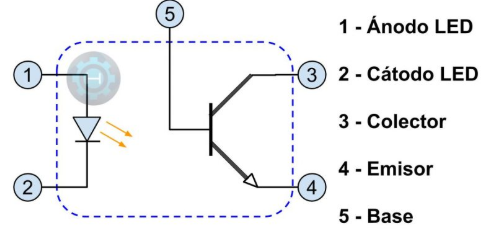
\includegraphics[scale=0.6]{Circuito/Opto.PNG}
\caption{Estructura del Optoacoplador}
\end{figure}

Relevador. \\
Un relevador es un aparato eléctrico que funciona como un interruptor pero que es accionado eléctricamente. El relé permite abrir o cerrar contactos mediante un electroimán, Fue desarrollado en la primera mitad del siglo XIX por el físico norteamericano Joseph Henry, a través de una bobina y un electroimán.
Lo que hace la bobina es crear un campo magnético que lleva los contactos a establecer una conexión. El electroimán, por su parte, permite el cierre de los contactos.
\begin{figure}[hbtp]
\centering
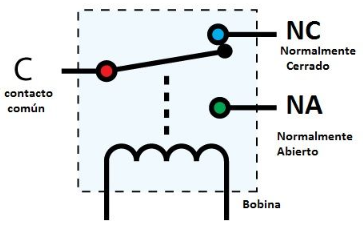
\includegraphics[scale=0.6]{Circuito/Rele.PNG}
\caption{Estructura del Relevador}
\end{figure}

\newpage
\section*{Materiales}
* Protoboard\\
* Cable para protoboard\\
* 3 Push button\\
* 3 Relevadores 5V\\
* 3 Optoacopladores 4N25\\
* Resistencias \\
* 3 Transistores 2N2222\\
* Arduino (en este caso Arduino UNO)

\section*{Equipo}
* Fuente de alimentación \\
* Laptop 

\section*{Programa}
* Arduino 

\newpage
\section{Desarrollo}
1. Dado el siguiente circuito, calcular el valor de las resistencias faltantes: 
\begin{figure}[hbtp]
\centering
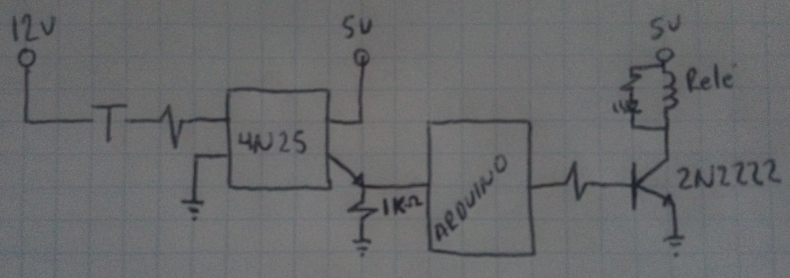
\includegraphics[scale=0.7]{Circuito/Circuito1.PNG}
\caption{Circuito PLC}
\end{figure}\\
Para calcular los valores de las 3 resistencias que nos hace falta debemos obtenerlas mediante el datasheet del optoacoplador y del transistor.

Sustituimos valores del datasheet del opto en la formula y obtendremos: 
\textbf{OPTO}\\
\\
LED(IR)\\
$V_f=1.15V$\\
$I_f=10mA$\\
\begin{equation}
LED=\frac{(12V-1.15V)}{10mA}=1085\Omega\\
\end{equation}

Sustituimos valores del datasheet del transistor en la formula y obtendremos:
\textbf{TRANSISTOR}\\
\begin{equation}
R=\frac{(5V-0.6V)*250}{12mA}=1528\Omega\\
\end{equation}
\\
$W_L=(1^2)R$\\
$W_L=(10mA)^2(1100\Omega)$\\
$W_L=0.11W$\\

Para la resistencia del LED investigamos en la web y nos salió que la resistencia que debemos colocar para 5V es dependiendo del tipo de LED, en nuestro caso utilizamos de 330 ohms y 660 ohms.\\

\newpage
Teniendo ya el circuito completo. 
\begin{figure}[hbtp]
\centering
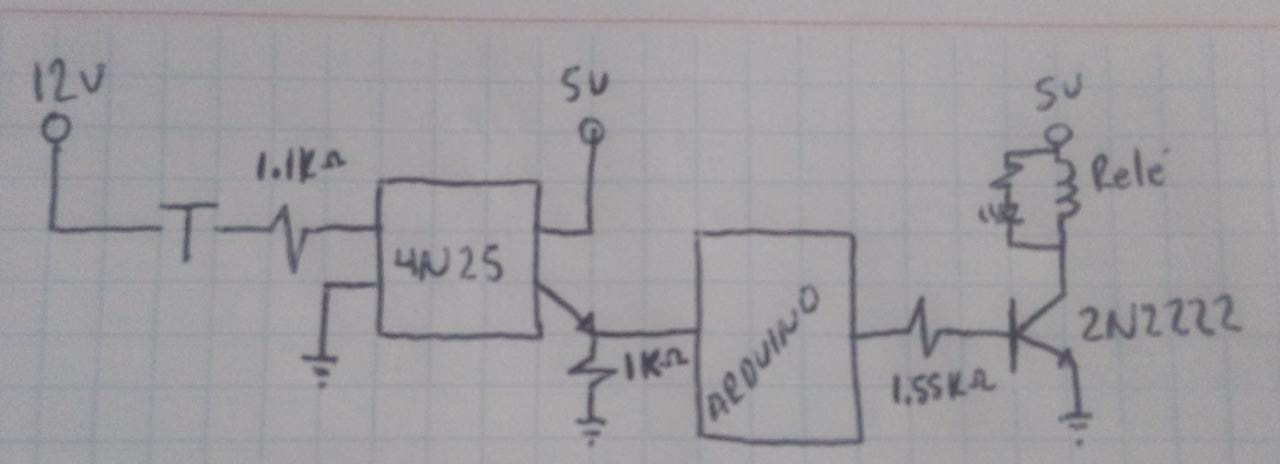
\includegraphics[scale=0.35]{Circuito/Circuito2.jpeg}
\caption{Circuito completo PLC}
\end{figure}

2. Armamos el circuito, teniendo en cuenta que debemos tener 3 entradas y 3 salidas como mínimo para tener nuestro circuito básico PLC, quedando: 
\begin{figure}[hbtp]
\centering
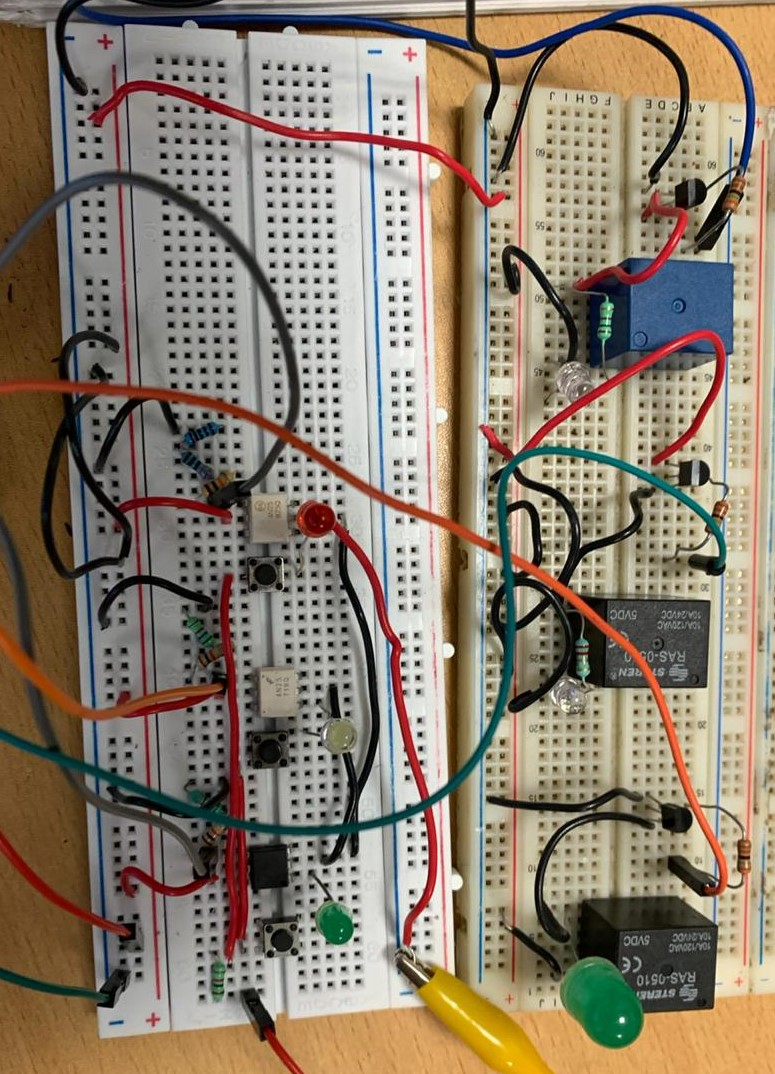
\includegraphics[scale=0.4]{Circuito/Circuito3.jpg}
\caption{Circuito armado}
\end{figure}

\newpage
3. Realizamos el programa de Arduino, teniendo en cuenta que cuando el Push Button se active, prenda el led y se active el relevador, obteniendo el siguiente programa: 

\begin{figure}[hbtp]
\centering
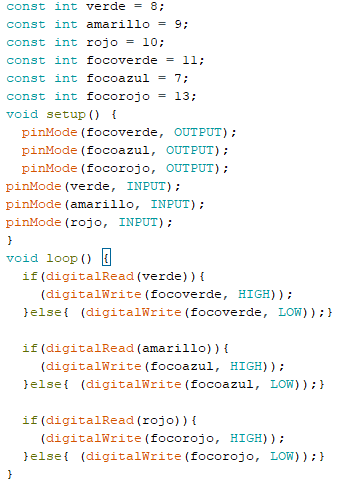
\includegraphics[scale=0.8]{Circuito/Arduino.png}
\caption{Programa Arduino}
\end{figure}

Una vez hecho el programa vamos a conectar los pines de entrada y salida como corresponden al circuito: 
\begin{figure}[hbtp]
\centering
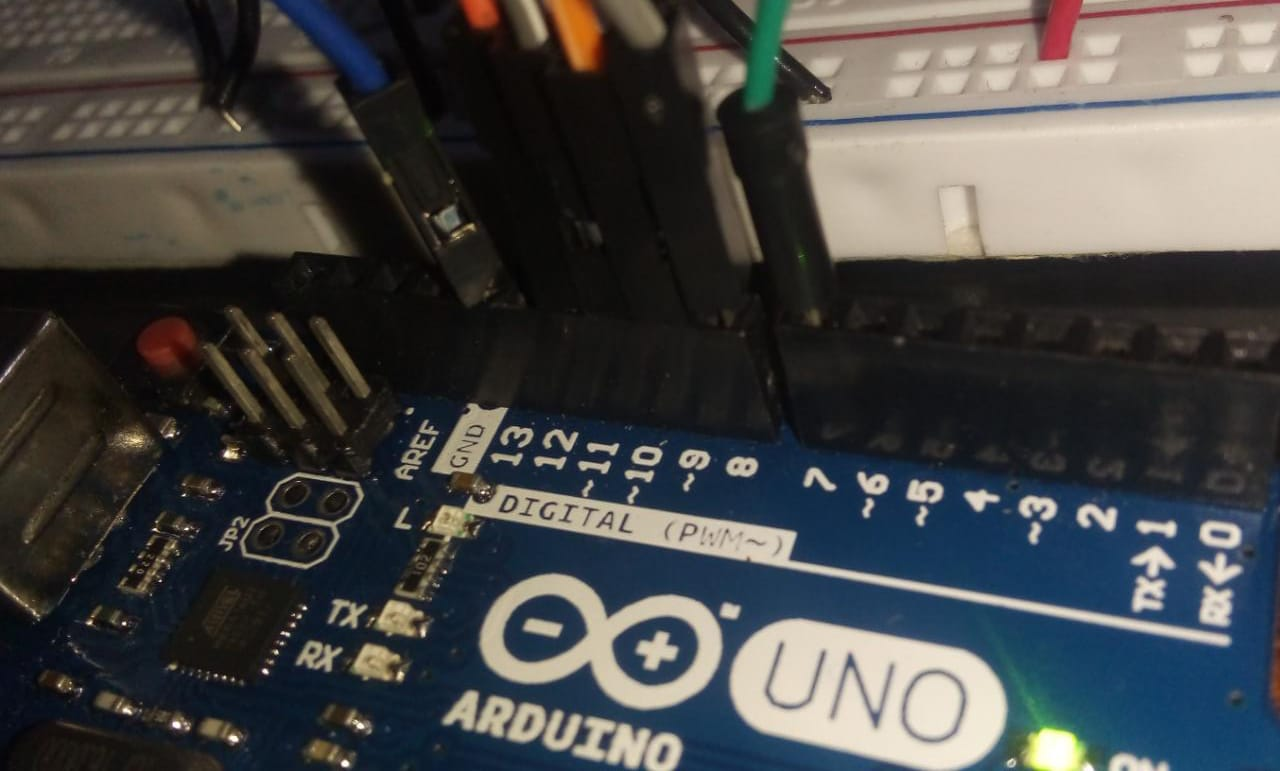
\includegraphics[scale=0.25]{Circuito/Arduino.jpeg}
\caption{Entradas y salidas del Arduino}
\end{figure}

\newpage
4. Conectamos el Arduino a la computadora, compilamos el programa y lo subimos para que se cargue en el Arduino, conectamos voltaje de 5V y 12V a los nodos correspondientes y echamos a funcionar el circuito.
\begin{figure}[hbtp]
\centering
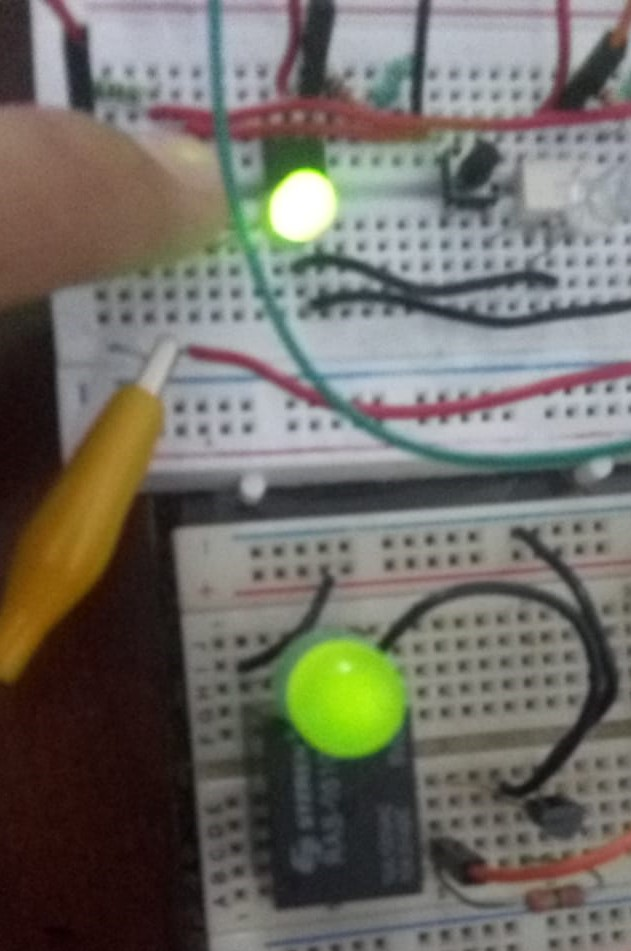
\includegraphics[scale=0.3]{Circuito/1.jpeg}
\caption{Entrada y salida No.1}
\end{figure}\\
Observamos que al activar el Push Button encienden dos leds, el primero es para comprobar que la corriente circula por el optoacoplador e indica que tenemos una entrada;el segundo indica que el relevador se activo, al igual debes escuchar el sonido que hace el relé cuando se activa, indicando que existe una salida.\\
\begin{figure}[hbtp]
\centering
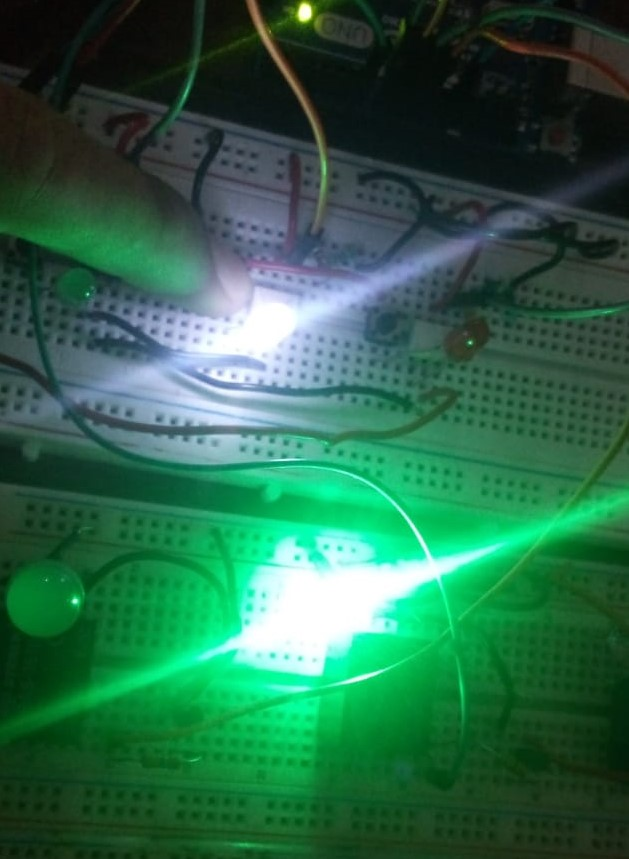
\includegraphics[scale=0.3]{Circuito/2.jpeg}
\caption{Entrada y salida No.2}
\end{figure}
\newpage
Al igual que la primera entrada, verificamos que tengamos una entrada y una salida en nuestro circuito.\\

\begin{figure}[hbtp]
\centering
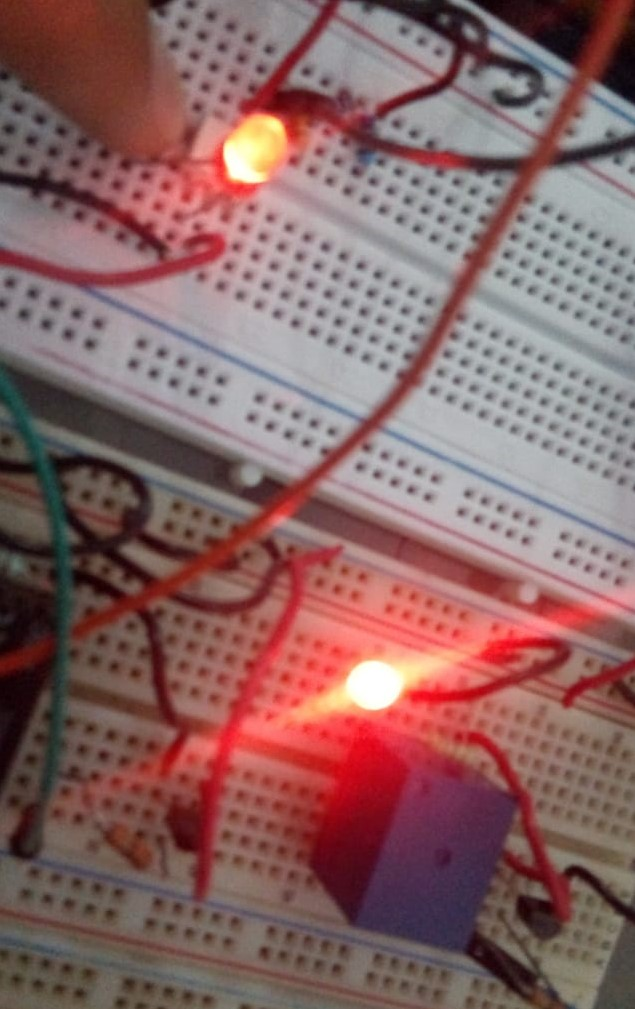
\includegraphics[scale=0.35]{Circuito/3.jpeg}
\caption{Entrada y salida No.3}
\end{figure} 
Observamos que nuestra práctica a resultado correctamente teniendo las 3 entradas y 3 salidas funcionando correctamente, teniendo nuestro PLC básico.

\newpage
\textbf{Conclusiones}\\
Ulises Isaac Reyes Alvarez.\\
La realización de esta práctica nos sirvió para aprender sobre el funcionamiento básico de un PLC, mediante 3 entradas y 3 salidas en nuestro caso, para ver su funcionamiento y como es su estructura. El PLC su funcionamiento principal es mediante una entrada hacer funcionar una salida mediante un micro controlador.\\
A mi no se me dificultó tanto el armar el circuito ya que la única falla que había era con el programa de Arduino, pero después de varios intentos resulto correctamente y funciono como debería de ser. \\

Luis Osvaldo Cervantes Martínez.\\
En esta ocasión la practica fue demasiado compleja, por lo que para mi fue demasiada complicada, ya que en el circuito nos salían fallas, las cuales corregíamos y salían nuevas fallas, tanto que necesitamos mas tiempo para poder complementarla.\\
Pero puedo resaltar el conocimiento obtenido, ya que en esta ocasión laboramos con elementos nuevos,por ejemplo, relevadores, optoacopladores, etc. Con lo que nos familiarizamos con el funcionamiento de un PLC, conocimos el funcionamiento de los relevadores y optoacopladores.\\ 
\newpage
\section{Referencias bibliográficas}
\url{https://hetpro-store.com/TUTORIALES/optoacoplador/}\\
\url{https://www.ingmecafenix.com/electricidad-industrial/relevador/}

\begin{figure}[hbtp]
\centering
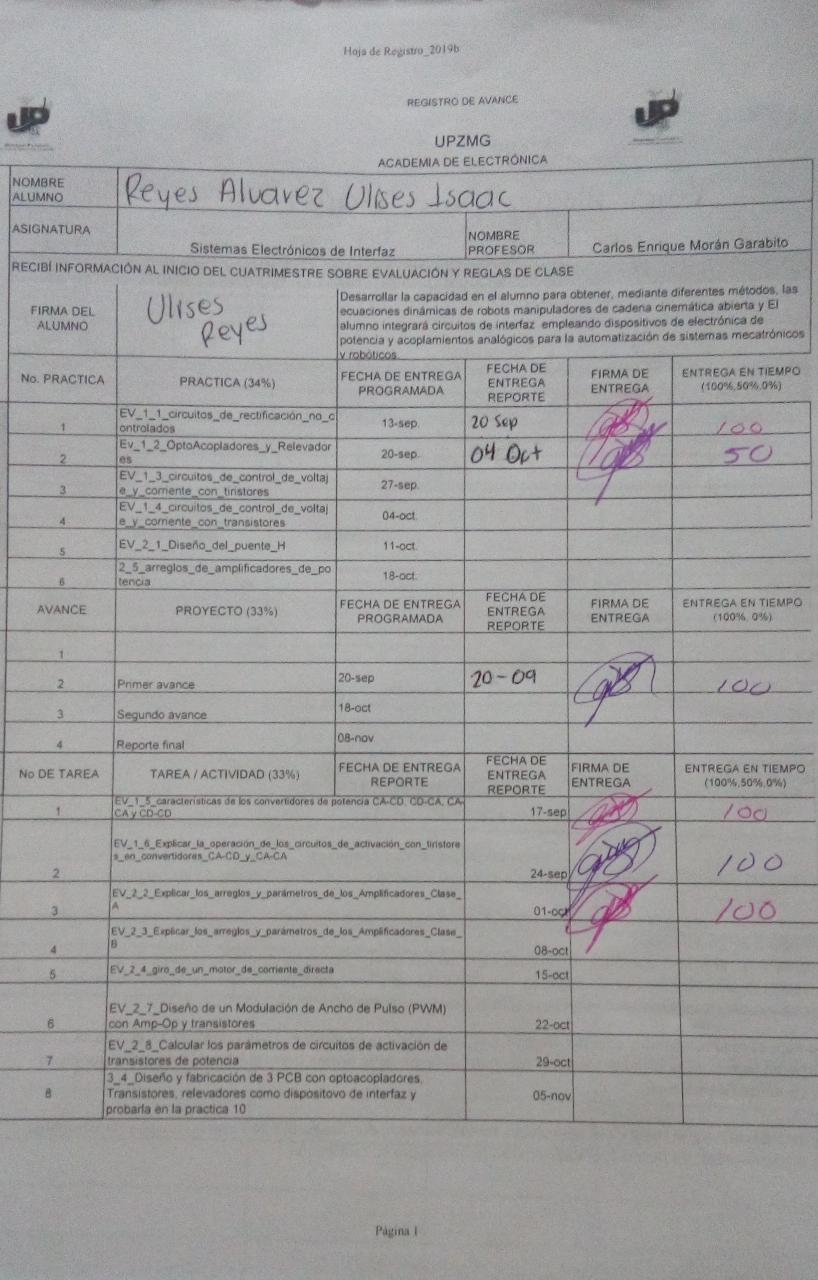
\includegraphics[scale=0.4]{Circuito/Firmas.jpeg}
\end{figure}



\end{document}